\documentclass[12pt,letterpaper,oneside]{report}
\usepackage[spanish]{babel}
\usepackage{fontspec}
\setmainfont{Times New Roman}
\setmonofont{Menlo}
\usepackage[letterpaper,margin=1in]{geometry}
\usepackage{setspace}
\onehalfspacing
\usepackage{graphicx}
\usepackage{float}
\usepackage{caption}
\usepackage{listings}
\usepackage{hyperref}
\usepackage{titlesec}
\usepackage{amsmath}

\titleformat{\chapter}[display]{\normalfont\bfseries\fontsize{24}{28}\selectfont}{}{0pt}{}
\titlespacing*{\chapter}{0pt}{0pt}{5pt}
\titlespacing*{\section}{0pt}{6pt}{3pt}
\hypersetup{colorlinks=true,linkcolor=black,urlcolor=black}
\captionsetup{font=small,justification=centering}
\setlength{\parindent}{0pt}
\setlength{\parskip}{6pt}
\renewcommand{\lstlistingname}{Código}

\lstset{
  basicstyle=\ttfamily\fontsize{9}{10}\selectfont,
  frame=single,
  numbers=left,
  numberstyle=\tiny,
  breaklines=true,
  columns=fullflexible,
  captionpos=b,
  showstringspaces=false
}

\begin{document}

\begin{titlepage}
\centering

\includegraphics[height=2.5in]{figuras/UAT-Escudo.jpeg}\par
\vspace{1.5cm}
{\bfseries\fontsize{16}{18}\selectfont Tarea 2\par}
\vspace{-0.2cm}
{\bfseries\fontsize{16}{18}\selectfont Programas e invariante de ciclo\par}
\vspace{1cm}
{\bfseries\fontsize{16}{18}\selectfont Análisis y Diseño de Algoritmos\par}
\vspace{-0.2cm}
{\bfseries\fontsize{16}{18}\selectfont Maestría en Ciencias e Ingeniería de Datos\par}
\vspace{1cm}
{\fontsize{14}{16}\selectfont Alumno: Rodrigo Piña Enríquez\par}
\vspace{-0.2cm}
{\fontsize{14}{16}\selectfont Profesor: Dr. José Lázaro Martínez Rodríguez\par}
\vfill

\includegraphics[height=0.7in]{figuras/FIC-03.png}\par
\vspace{0.5cm}
{\fontsize{14}{16}\selectfont Septiembre 2026\par}
\end{titlepage}

\tableofcontents
\clearpage

\chapter*{Introducción}
\addcontentsline{toc}{chapter}{Introducción}

En esta tarea se implementan tres algoritmos iterativos en Rust: el ordenamiento
por inserción ascendente, su variante descendente y la suma de dos números
binarios almacenados en arreglos. Además, se presenta una prueba de escritorio
del algoritmo Insertion Sort y una síntesis sobre el invariante de ciclo y la
correctez de algoritmos iterativos, con base en los materiales audiovisuales
proporcionados.

\clearpage
\chapter*{1. Insertion Sort}
\addcontentsline{toc}{chapter}{1. Insertion Sort}
\setcounter{chapter}{1}
\setcounter{section}{0}

\section*{1.1 Ascendente}
\addcontentsline{toc}{section}{1.1 Ascendente}
\setcounter{section}{1}
\setcounter{subsection}{0}

\subsection{Enunciado}

Implementar Insertion Sort de acuerdo con el pseudocódigo compartido en clase,
en el lenguaje de programación de preferencia.

\subsection{Pseudocódigo}

\begin{lstlisting}[caption={Pseudocódigo de Insertion Sort Ascendente},label={pseudo:insertion-asc}]
Insertion Sort Asc(A)
    for j = 1 to longitud(A) - 1
        clave = A[j]
        i = j - 1
        while i >= 0 and A[i] > clave
            A[i + 1] = A[i]
            i = i - 1
        A[i + 1] = clave
    return A
\end{lstlisting}

\subsection{Código desarrollado}

\lstinputlisting[
  firstline=1,
  lastline=14,
  caption={Implementación de Insertion Sort Ascendente en Rust},
  label={cod:insertion-asc}
]{../algoritmos/src/insertion.rs}

\clearpage

\subsection{Prueba de escritorio}

La Tabla \ref{tab:prueba-escritorio} muestra la traza del arreglo solicitado
$A=[31,41,59,26,41,58]$. En cada iteración se inserta la clave en la parte
izquierda, que permanece ordenada.

\begin{table}[H]
\centering
\caption{Prueba de escritorio de Insertion Sort ascendente}
\label{tab:prueba-escritorio}

\begin{tabular}{c|c|l}
Iteración & Clave & Arreglo después de insertar la clave \\ \hline
Inicial & -- & [31, 41, 59, 26, 41, 58] \\
1 & 41 & [31, 41, 59, 26, 41, 58] \\
2 & 59 & [31, 41, 59, 26, 41, 58] \\
3 & 26 & [26, 31, 41, 59, 41, 58] \\
4 & 41 & [26, 31, 41, 41, 59, 58] \\
5 & 58 & [26, 31, 41, 41, 58, 59] \\
\end{tabular}
\end{table}

\subsection{Prueba de ejecución}

\begin{figure}[H]
\centering
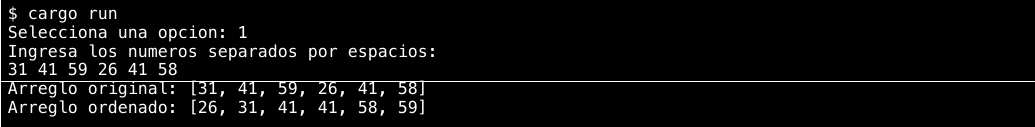
\includegraphics[width=\textwidth]{figuras/pruebas/insertion_ascendente.png}
\caption{Ejecución de Insertion Sort Ascendente con el arreglo indicado.}
\label{fig:insertion-asc}
\end{figure}

\clearpage
\section*{1.2 Descendente}
\addcontentsline{toc}{section}{1.2 Descendente}
\setcounter{section}{2}
\setcounter{subsection}{0}

\subsection{Enunciado}

Reescribir Insert Sort para ordenar de forma descendente.

\subsection{Pseudocódigo}

\begin{lstlisting}[caption={Pseudocódigo de Insertion Sort Descendente},label={pseudo:insertion-desc}]
Insertion Sort Desc(A)
    for j = 1 to longitud(A) - 1
        clave = A[j]
        i = j - 1
        while i >= 0 and A[i] < clave
            A[i + 1] = A[i]
            i = i - 1
        A[i + 1] = clave
    return A
\end{lstlisting}

\subsection{Código desarrollado}

\lstinputlisting[
  firstline=16,
  lastline=29,
  caption={Implementación de INSERTION-SORT descendente en Rust},
  label={cod:insertion-desc}
]{../algoritmos/src/insertion.rs}

\subsection{Prueba de ejecución}

\begin{figure}[H]
\centering
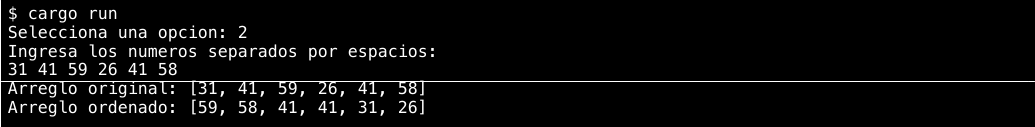
\includegraphics[width=\textwidth]{figuras/pruebas/insertion_descendente.png}
\caption{Ejecución de INSERTION-SORT descendente.}
\label{fig:insertion-desc}
\end{figure}

\section{Prueba de escritorio manual}

\begin{figure}[H]
\centering
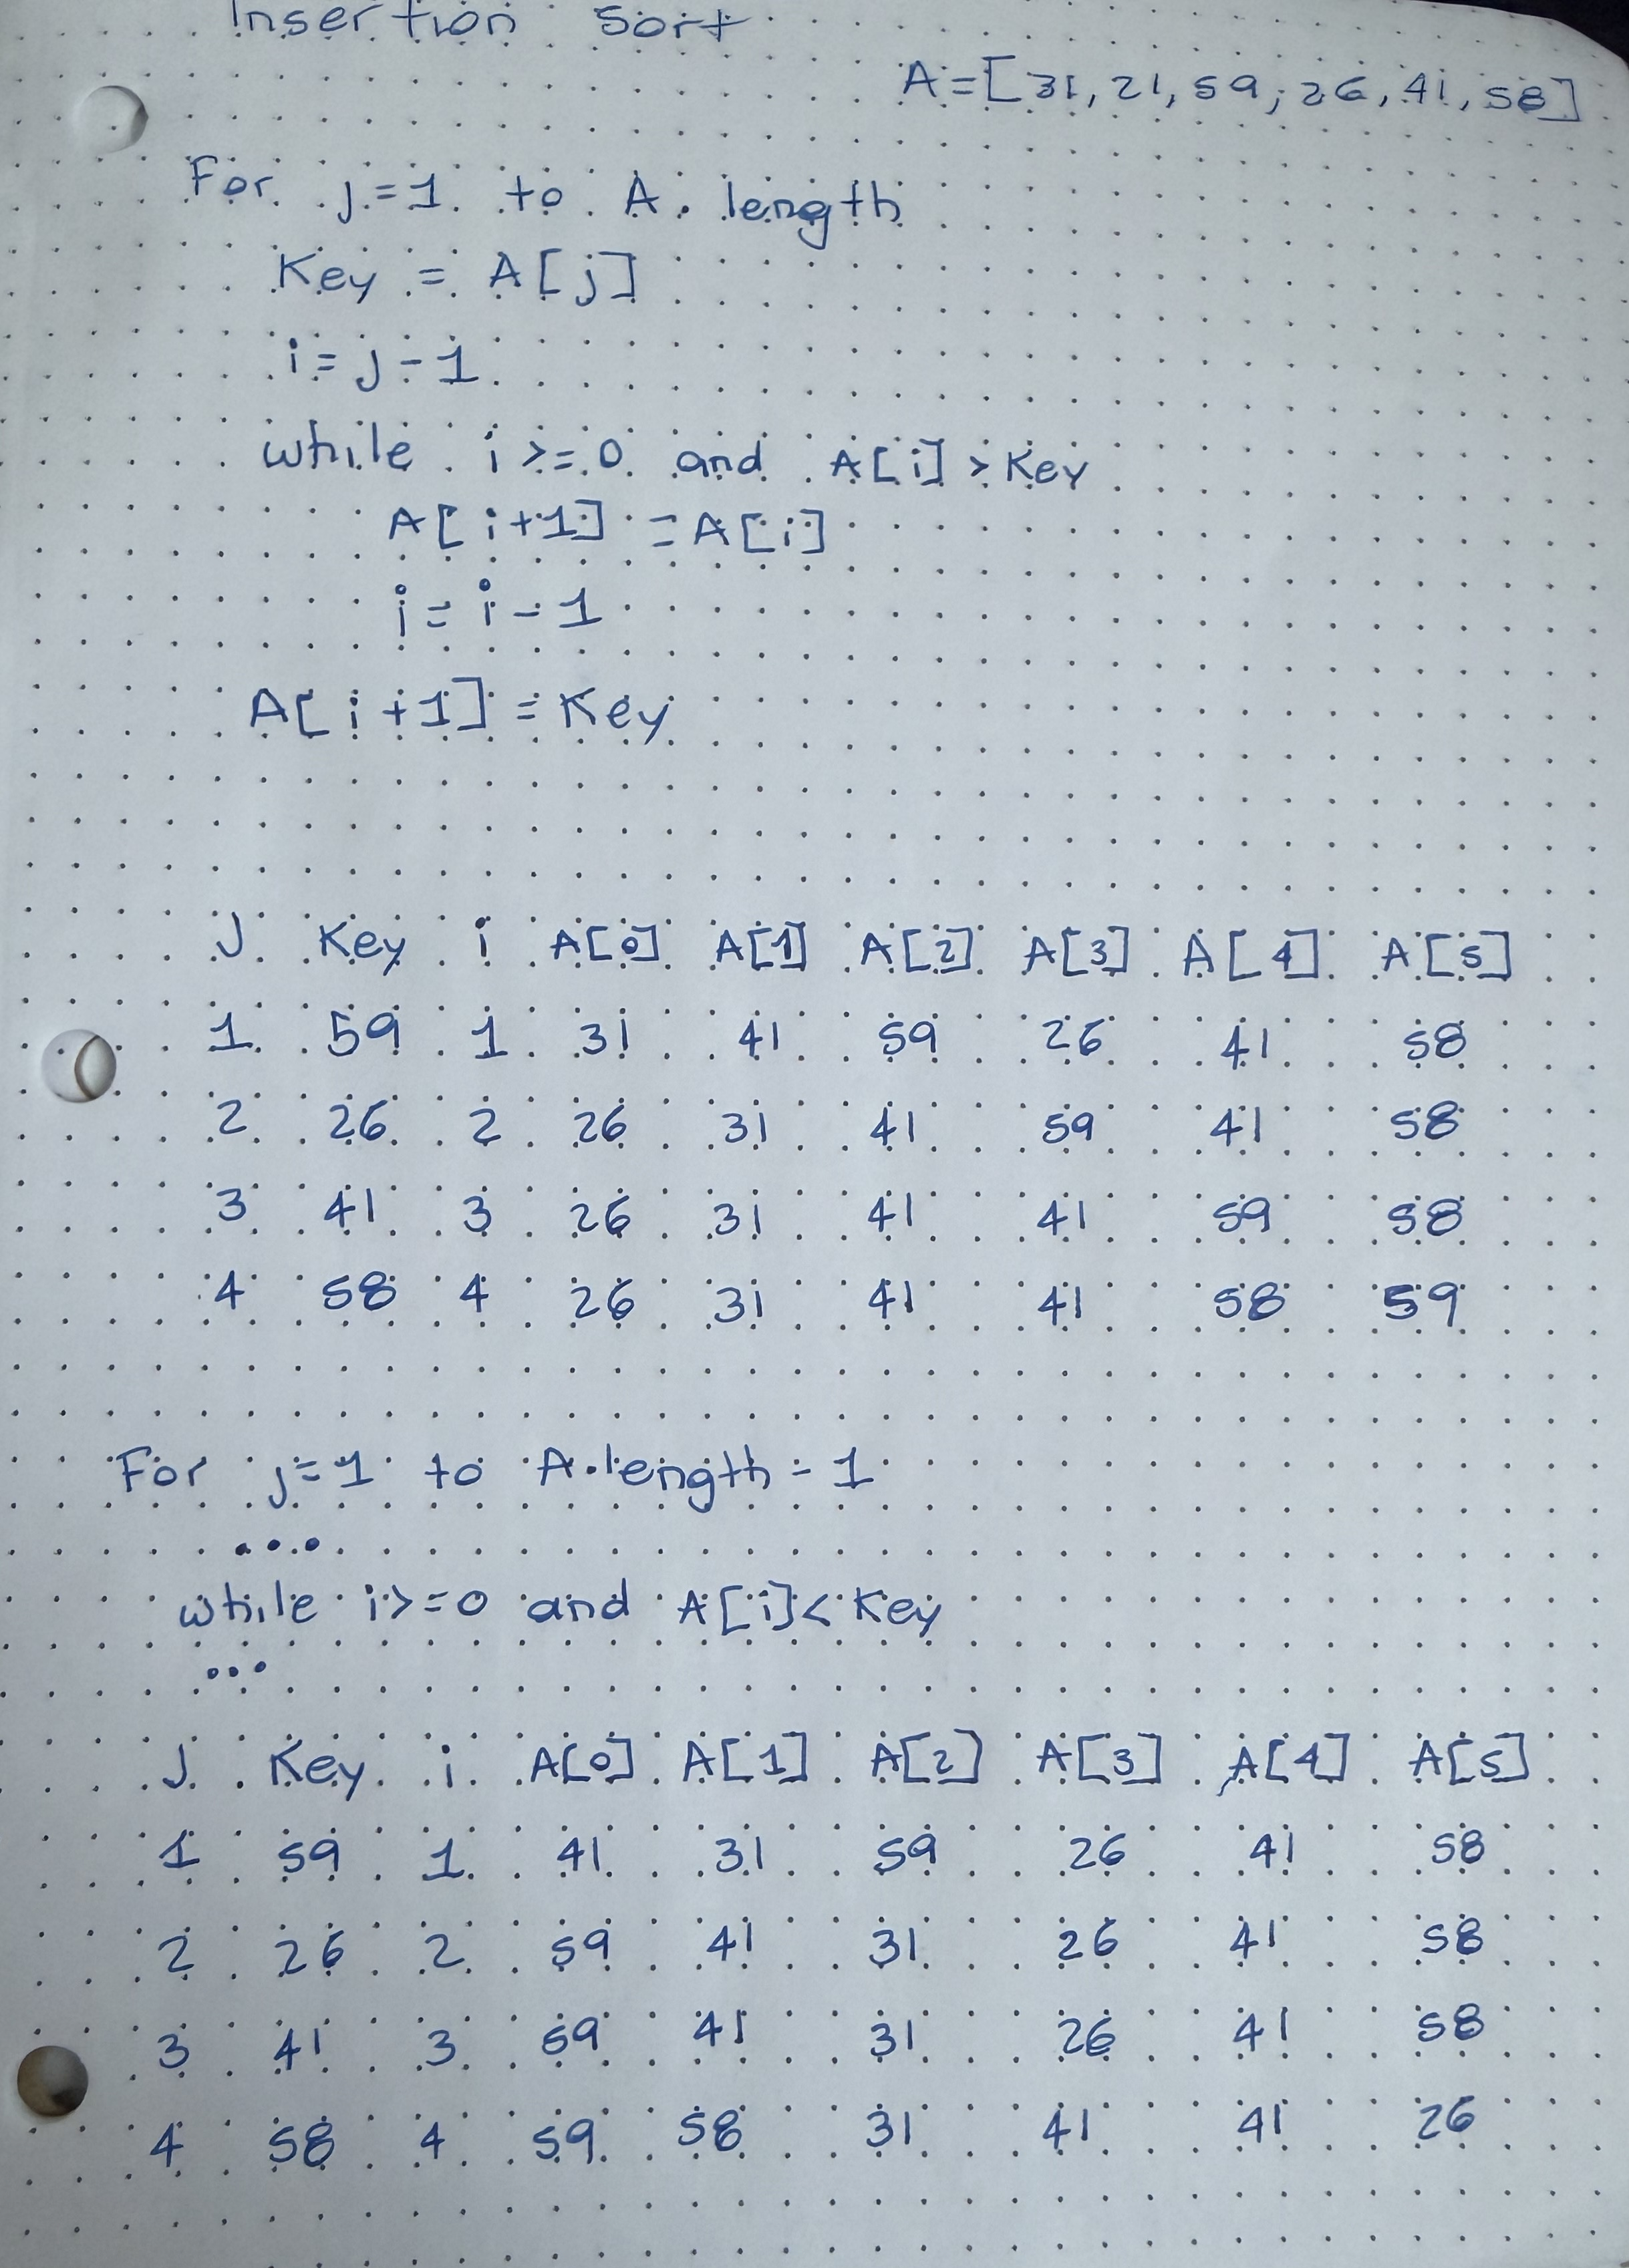
\includegraphics[angle=-90,origin=c,width=0.55\textheight]{figuras/pruebas/prueba_escritorio.jpeg}
\caption{Prueba de escritorio realizada manualmente para INSERTION-SORT.}
\label{fig:prueba-escritorio-manual}
\end{figure}

\clearpage
\chapter*{2. Suma de números binarios}
\addcontentsline{toc}{chapter}{2. Suma de números binarios}
\setcounter{chapter}{2}
\setcounter{section}{0}

\section{Enunciado}

Desarrollar un algoritmo para sumar dos números binarios de $n$ bits almacenados
en dos arreglos $A$ y $B$ de $n$ elementos. La suma se almacena en forma binaria
en un arreglo de $n+1$ elementos.

\section{Declaración formal del problema}

Sean $A=(a_0,a_1,\ldots,a_{n-1})$ y $B=(b_0,b_1,\ldots,b_{n-1})$, donde
$a_i,b_i \in \{0,1\}$. Se requiere construir
$C=(c_0,c_1,\ldots,c_n)$ tal que el valor binario de $C$ sea igual a la suma de
los valores binarios representados por $A$ y $B$. El bit $c_0$ almacena el
acarreo final.

\section{Pseudocódigo}

\begin{lstlisting}[caption={Pseudocódigo para la suma de dos arreglos binarios},label={pseudo:binarios}]
Suma Binaria(A, B)
    n = longitud(A)
    crear C[0..n] con ceros
    acarreo = 0
    for i = n - 1 downto 0
        suma = A[i] + B[i] + acarreo
        C[i + 1] = suma mod 2
        acarreo = suma div 2
    C[0] = acarreo
    return C
\end{lstlisting}
\clearpage
\section{Código desarrollado}

\lstinputlisting[
  caption={Implementación de la suma binaria en Rust},
  label={cod:binarios}
]{../algoritmos/src/binary.rs}

\section{Prueba de ejecución}

Se utilizaron $A=1011$ y $B=0110$. La suma binaria obtenida es $10001$.

\begin{figure}[H]
\centering
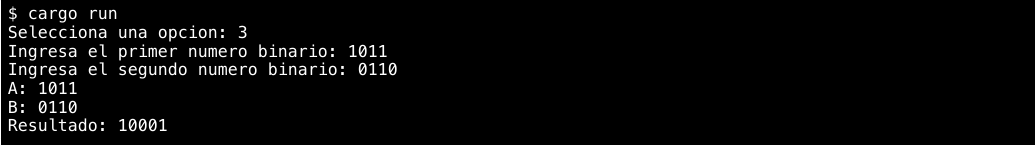
\includegraphics[width=\textwidth]{figuras/pruebas/suma_binaria.png}
\caption{Ejecución de la suma de dos números binarios de cuatro bits.}
\label{fig:suma-binaria}
\end{figure}

\clearpage
\chapter*{3. Invariante de ciclo y correctez}
\addcontentsline{toc}{chapter}{3. Invariante de ciclo y correctez}
\setcounter{chapter}{3}
\setcounter{section}{0}

\section{Invariante de ciclo}

Un invariante de ciclo es una propiedad que se cumple antes de iniciar un ciclo,
se conserva después de cada iteración y permite demostrar el resultado cuando el
ciclo termina. Para construirlo es necesario identificar qué información debe
permanecer verdadera durante la ejecución y relacionarla con el objetivo final
del algoritmo.

En el video sobre la técnica del invariante se utiliza el cálculo iterativo del
factorial. Si $n_0$ es el valor inicial, durante el ciclo se mantienen las
propiedades $n>0$ y $f=\frac{n_0!}{n!}$. La condición $n>0$ garantiza que el
factorial de $n$ está definido y que todavía existen factores por procesar. La
segunda propiedad relaciona el producto parcial almacenado en $f$ con los
factores que aún faltan por multiplicar.

\begin{figure}[H]
\centering
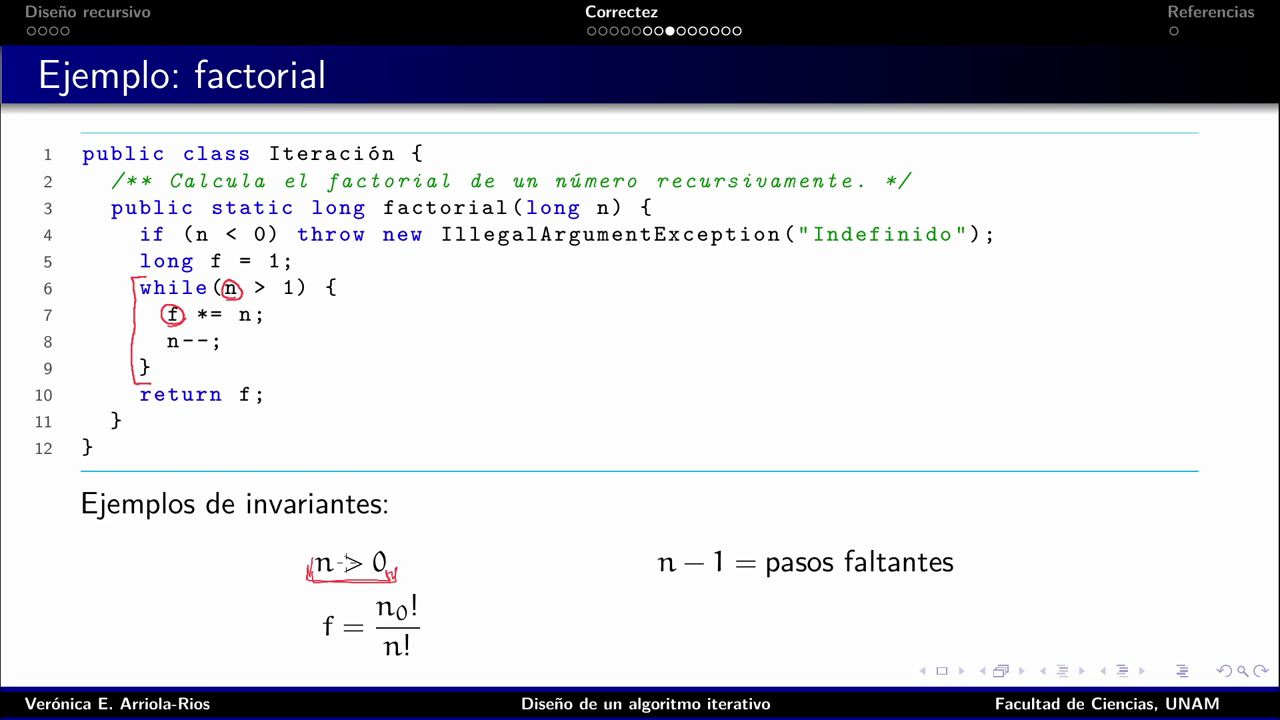
\includegraphics[width=0.9\textwidth]{figuras/invariante/factorial_invariante.png}
\caption{Ejemplo de invariantes en el algoritmo iterativo para calcular factorial.}
\label{fig:factorial-invariante}
\end{figure}

\begin{figure}[H]
\centering
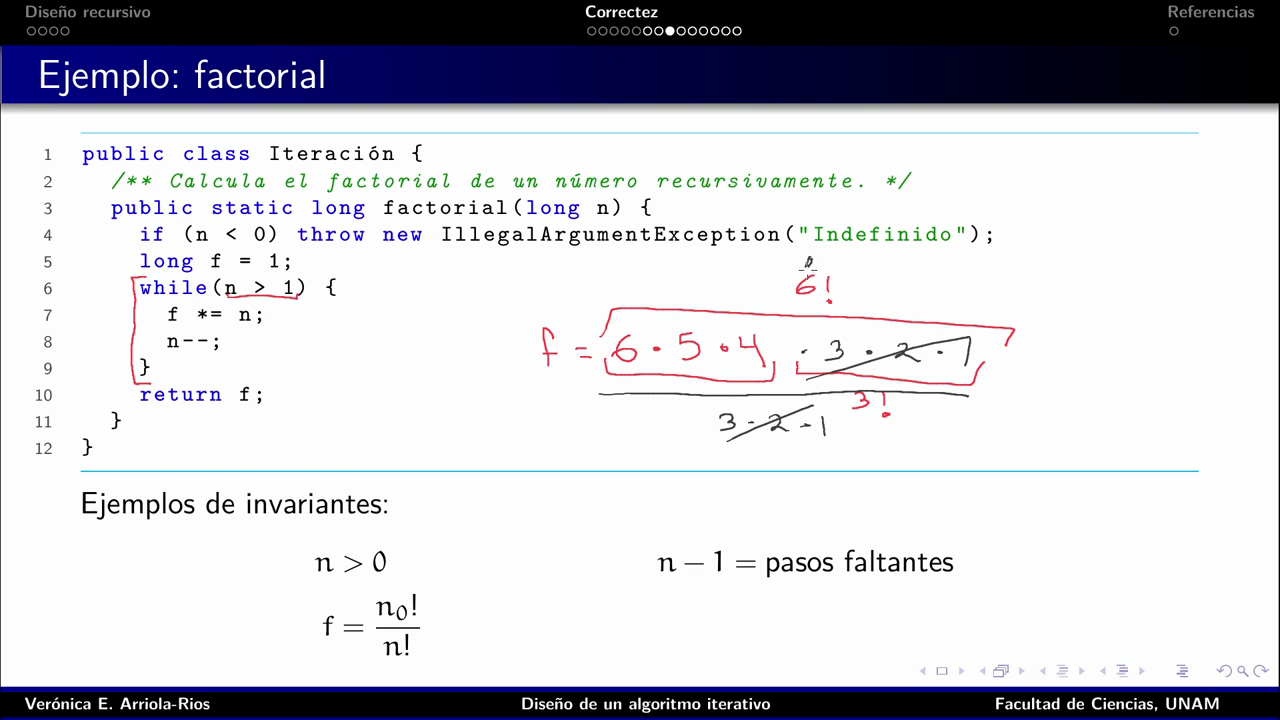
\includegraphics[width=0.9\textwidth]{figuras/invariante/ejemplo_factorial.png}
\caption{Desarrollo paso a paso del producto parcial en el ejemplo de factorial.}
\label{fig:ejemplo-factorial}
\end{figure}

\section{Correctez de un algoritmo iterativo}

La correctez de un algoritmo iterativo se argumenta mediante tres componentes:

\begin{enumerate}
\item \textbf{Inicialización.} Se verifica que el invariante sea verdadero
antes de la primera iteración.
\item \textbf{Mantenimiento.} Se demuestra que, si el invariante es verdadero
al inicio de una iteración, continúa siéndolo después de ejecutar el cuerpo del
ciclo.
\item \textbf{Terminación.} Se usa la condición que detiene el ciclo junto con
el invariante para concluir que se alcanzó el resultado requerido.
\end{enumerate}

En el ejemplo del factorial, el caso base inicia con $f=1$ y $n=n_0$, por lo
que $f=\frac{n_0!}{n_0!}=1$. En el paso inductivo se ejecutan dos operaciones:
primero $f' = f\cdot n$ y después $n'=n-1$. Al sustituir el invariante se
obtiene $f'=n\cdot\frac{n_0!}{n!}=\frac{n_0!}{(n-1)!}
=\frac{n_0!}{n'!}$; por tanto, la propiedad permanece verdadera. Cuando el
ciclo termina, ya no quedan factores pendientes y el valor acumulado
corresponde a $n_0!$.

\begin{figure}[H]
\centering
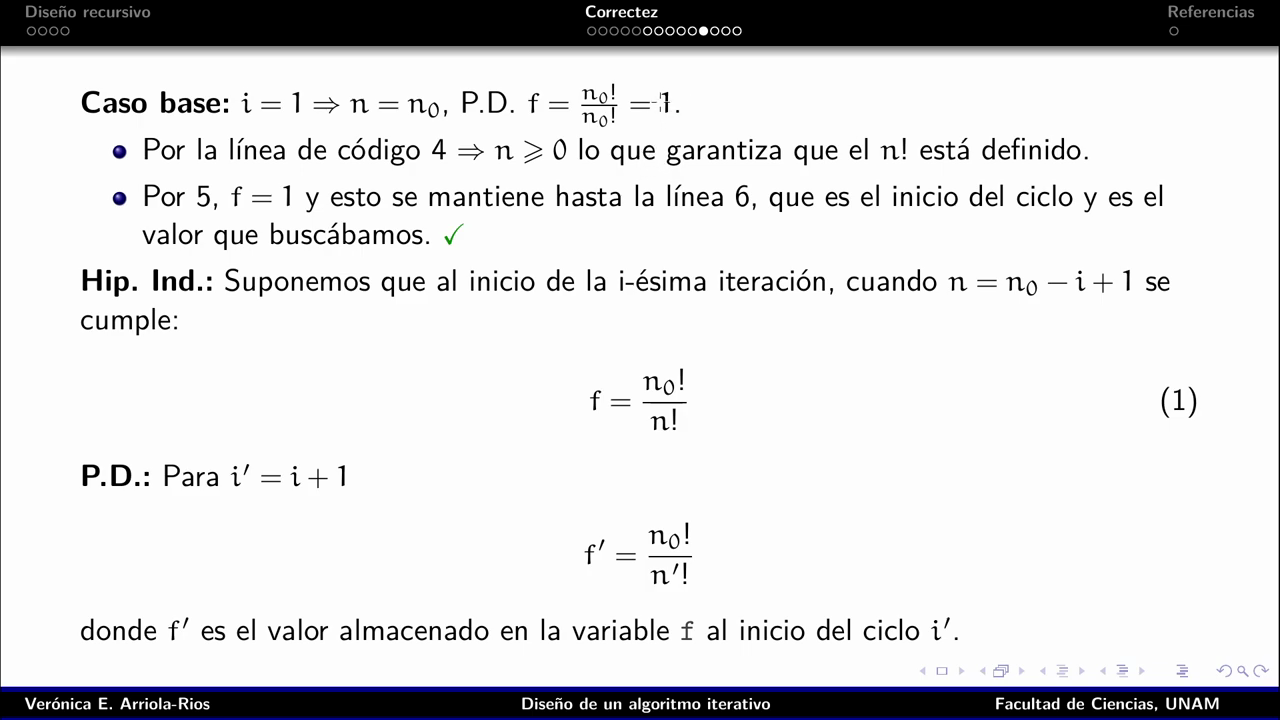
\includegraphics[width=0.9\textwidth]{figuras/invariante/caso_base_induccion.png}
\caption{Caso base e hipótesis inductiva mostrados en el video de correctez.}
\label{fig:caso-base}
\end{figure}

\begin{figure}[H]
\centering
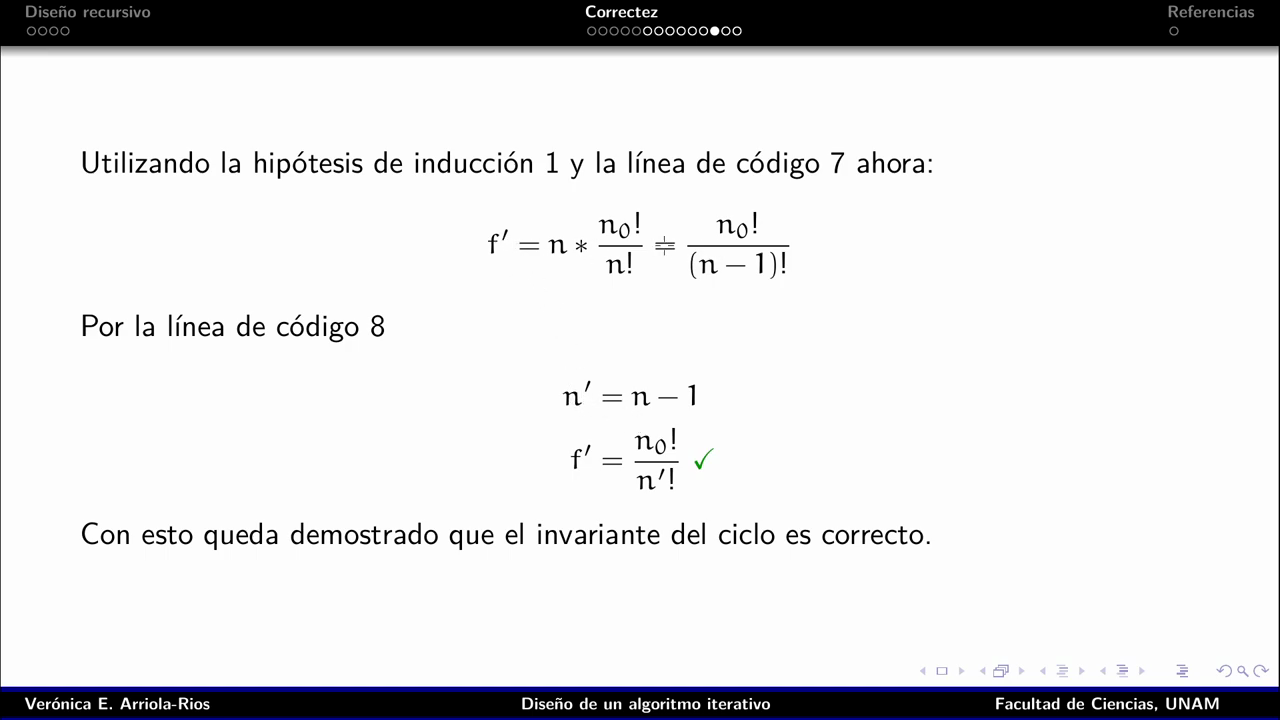
\includegraphics[width=0.9\textwidth]{figuras/invariante/paso_inductivo.png}
\caption{Paso inductivo para conservar el invariante del factorial.}
\label{fig:paso-inductivo}
\end{figure}
\clearpage
\section{Aplicación paso por paso a Insertion Sort}

En Insertion Sort, el ciclo exterior utiliza el índice $j$ para seleccionar la
clave que se insertará. El invariante es el siguiente: \textit{al inicio de cada
iteración con índice $j$, el subarreglo $A[0..j-1]$ está ordenado y contiene
exactamente los mismos elementos que ocupaban esas posiciones en el arreglo
original}.

\begin{enumerate}
\item \textbf{Inicialización.} Antes de la primera iteración, $j=1$. El
subarreglo $A[0..0]$ tiene un solo elemento, por lo tanto ya está ordenado y el
invariante es verdadero.
\item \textbf{Mantenimiento.} Se guarda $A[j]$ en la variable \texttt{key}.
Mientras el elemento situado a la izquierda sea mayor que la clave, se desplaza
una posición a la derecha. Cuando se detiene el ciclo interno, la clave se coloca
en la posición libre. Así, $A[0..j]$ queda ordenado y conserva los mismos
elementos que antes de la iteración.
\item \textbf{Terminación.} El ciclo exterior termina cuando $j$ alcanza la
longitud del arreglo. En ese momento el subarreglo ordenado es todo $A$, de modo
que el algoritmo devuelve una permutación ordenada de los elementos originales.
\end{enumerate}

La variante descendente utiliza el mismo razonamiento; únicamente cambia la
comparación del ciclo interno para desplazar los elementos menores que la clave.

\section{Aplicación paso por paso a la Suma Binaria}

Para sumar los arreglos binarios, el ciclo recorre los bits de derecha a
izquierda. El invariante es: \textit{al inicio de la iteración de índice $i$,
las posiciones $C[i+1..n]$ ya contienen la suma correcta de los bits procesados
de $A$ y $B$, y \texttt{carry} contiene el acarreo que debe sumarse en la
posición $i$}.

\begin{enumerate}
\item \textbf{Inicialización.} Antes de procesar el bit menos significativo,
el arreglo resultado contiene ceros y \texttt{carry}$=0$. No se ha procesado
ningún bit, por lo que el invariante se cumple de forma vacía.
\item \textbf{Mantenimiento.} En cada posición se calcula
\texttt{sum = A[i] + B[i] + carry}. El residuo de dividir entre dos,
\texttt{sum mod 2}, se almacena en $C[i+1]$; el cociente,
\texttt{sum div 2}, se convierte en el nuevo acarreo. Por ello, la parte ya
procesada del resultado permanece correcta.
\item \textbf{Terminación.} Cuando se han procesado los $n$ bits, el único
valor pendiente es el acarreo final. Al asignarlo a $C[0]$, el arreglo de
$n+1$ posiciones representa exactamente la suma de los dos números binarios.
\end{enumerate}

\clearpage
\chapter*{Conclusiones}
\addcontentsline{toc}{chapter}{Conclusiones}

La implementación de \textbf{Insertion Sort} permitió comprobar el ordenamiento de un
arreglo tanto de forma ascendente como descendente. La prueba de escritorio
evidencia cómo cada clave se inserta en una región izquierda ya ordenada. La \textbf{Suma
Binaria} muestra el manejo explícito del acarreo y la necesidad de un bit
adicional en el resultado.

El análisis de invariante de ciclo proporciona una forma ordenada de justificar
la correctez de algoritmos iterativos. La inicialización, el mantenimiento y la
terminación permiten pasar de una observación sobre cada iteración a una
conclusión sobre el resultado total. En \textbf{Insertion Sort}, este razonamiento explica
por qué el arreglo queda ordenado al finalizar.

\chapter*{Material audiovisual consultado}
\addcontentsline{toc}{chapter}{Material audiovisual consultado}

Arriola-Ríos, V. Técnica del invariante de ciclo. Video proporcionado para la
tarea: \url{https://www.youtube.com/watch?v=jdrgmA-fcJo}

Arriola-Ríos, V. Correctez de un algoritmo iterativo. Video proporcionado para
la tarea: \url{https://www.youtube.com/watch?v=_foQWmiZmUo}

\chapter*{Repositorio del proyecto}
\addcontentsline{toc}{chapter}{Repositorio del proyecto}

El código fuente, el reporte en \LaTeX{} y los archivos correspondientes a la Tarea 2 se encuentran disponibles en el siguiente repositorio de GitHub:

\url{https://github.com/falconmutant/mcdi_algoritmos}

\end{document}
